\documentclass[a4paper,11pt]{jsarticle}


% 数式
\usepackage{amsmath,amsfonts}
\usepackage{bm}
% 画像
\usepackage[dvipdfmx]{graphicx}


%リンクの埋め込み
\usepackage[dvipdfmx]{hyperref}
%ソースコード
\usepackage{listings}

%図の位置の操作
\usepackage{float}


\renewcommand{\figurename}{Fig.}
\renewcommand{\tablename}{Table}

\lstset{frame=single,numbers=left,tabsize=2}
\begin{document}

\begin{titlepage}
%
\vspace*{-100pt}\noindent 
{\Large 制御工学特論 中間レポート 12月5~12日提出ver}\vspace{5pt} \par
2023年 12月11日   \vspace{5pt} \par
%
\begin{tabular}{@{}ll}
氏名  & 山崎 楓        \\
学籍番号 & 6300607\\
名列 & 1M1-66\\
学部  & 工学研究科 機械工学専攻
\end{tabular}
%
\end{titlepage}

\section{オドメトリの評価実験}
本実験では,ルンバ600シリーズを用いて実験を行う.ルンバ600シリーズは差動二輪駆動のロボットであり,シリアル通信で
操縦とセンサ情報を取得することが可能である.
本実験ではルンバのエンコーダーより取得した両車輪の回転角度よりオドメトリを行い,ルンバの姿勢と位置を算出し,オドメトリの精度を評価する.
実験で用いたプログラムは以下のリンクより確認されたい.
\href{https://github.com/KIT-Robot2023/Roomba2023/tree/group1_shinomiya}{実験で用いたプログラム Group1Shinomiya}

\subsection{実験方法}
次に実験方法について説明する.まず,ルンバの上にモーションキャプチャー用のマーカーを5つ取り付ける.
その後,モーションキャプチャにおける中心座標にルンバを設置し動作させる.動作中は,オドメトリで算出された自己位置と姿勢を記録しながら,
モーションキャプチャーカメラでも移動中のルンバの座標を記録する.
計測後はモーションキャプチャーカメラで取得した座標を真値として,オドメトリで算出した自己位置と姿勢を評価する.\\
本実験で計測したルンバの動作は,直進とその場旋回である.


\subsection{結果}
Fig.1にルンバの直進動作におけるオドメトリ座標と真値の推移を示し,Fig.2に直進動作におけるオドメトリによるルンバの姿勢と真値のおける姿勢を示す.
また,Fig.3にルンバの旋回動作におけるオドメトリ座標と真値の推移を示し,Fig.4に旋回動作におけるオドメトリによるルンバの姿勢と真値のおける姿勢を示す.
ここで,Fig.1においては,x軸の正方向が進行方向である.

\begin{figure}[H]\centering
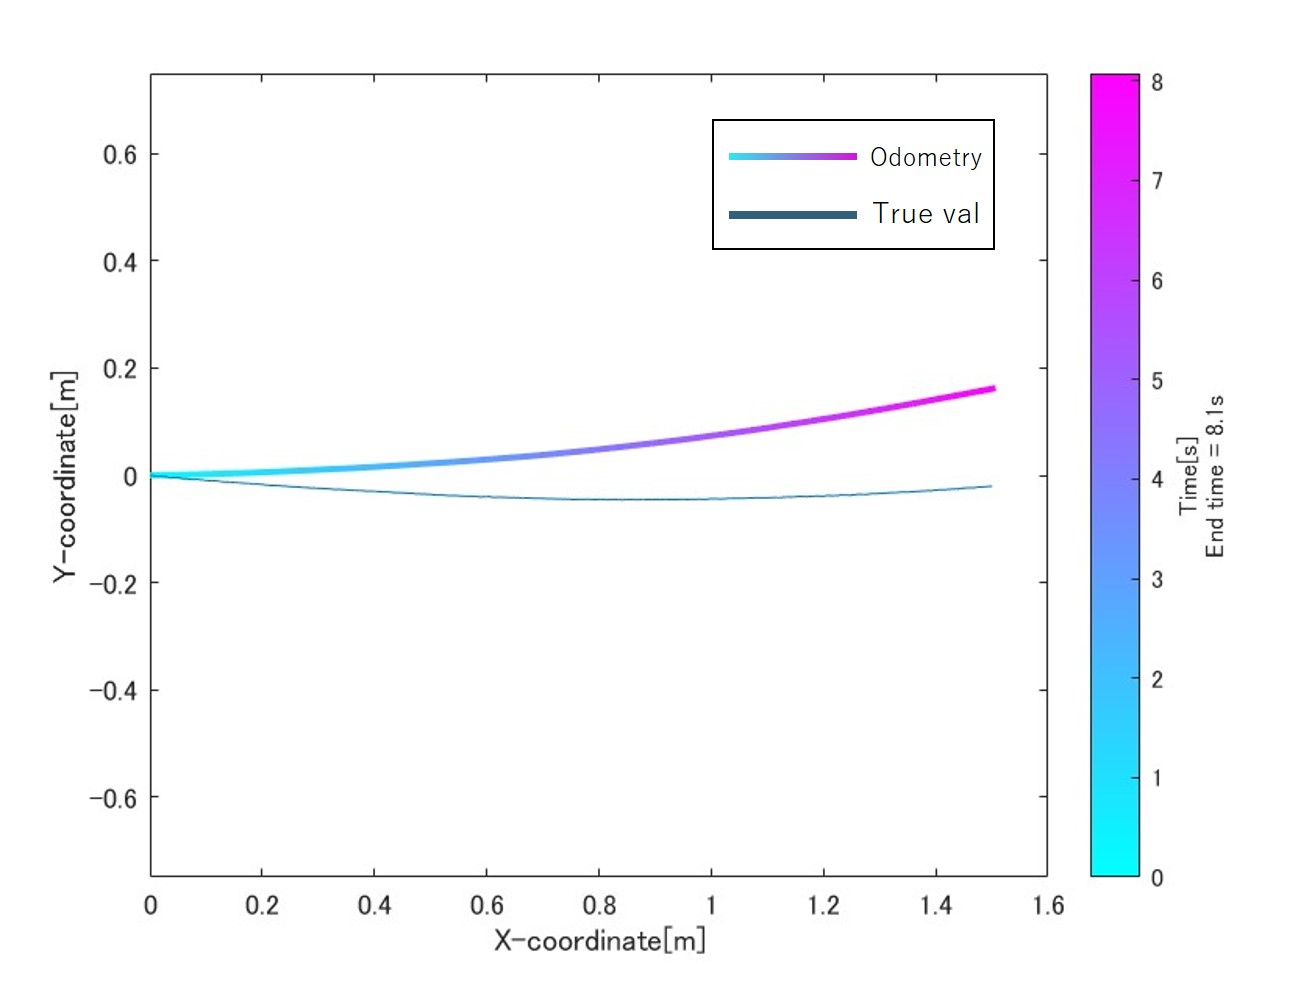
\includegraphics[width=100mm]{fig_1_2.jpg}
\caption{Movement on a plane}
\label{fig:1}\vspace{0zh}\end{figure}

\begin{figure}[H]\centering
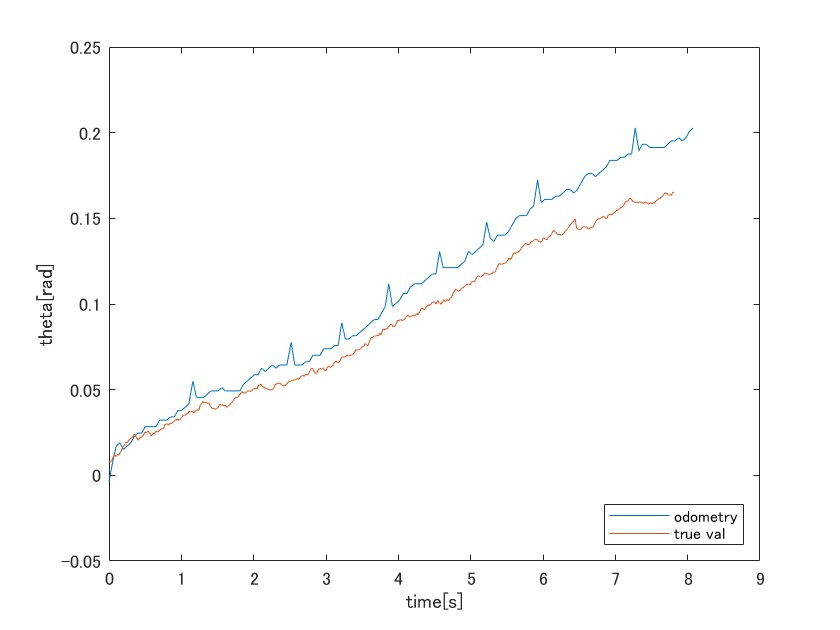
\includegraphics[width=100mm]{fig_2.jpg}
\caption{Angle Transition in Movement on a plane}
\label{fig:2}\vspace{0zh}\end{figure}

% \begin{figure}[H]\centering
% 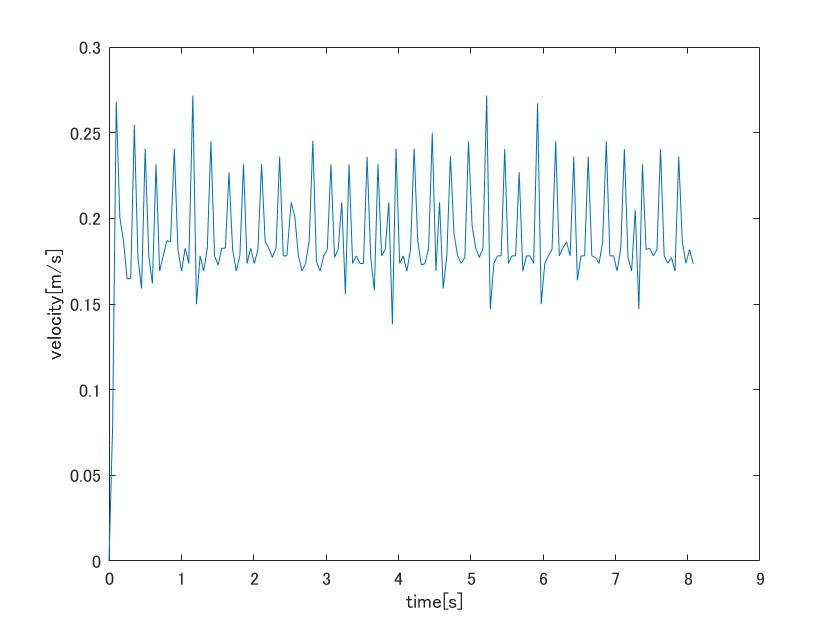
\includegraphics[width=100mm]{fig_5.jpg}
% \caption{Velocity in Movement on a plane}
% \label{fig:3}\vspace{0zh}\end{figure}

\begin{figure}[H]\centering
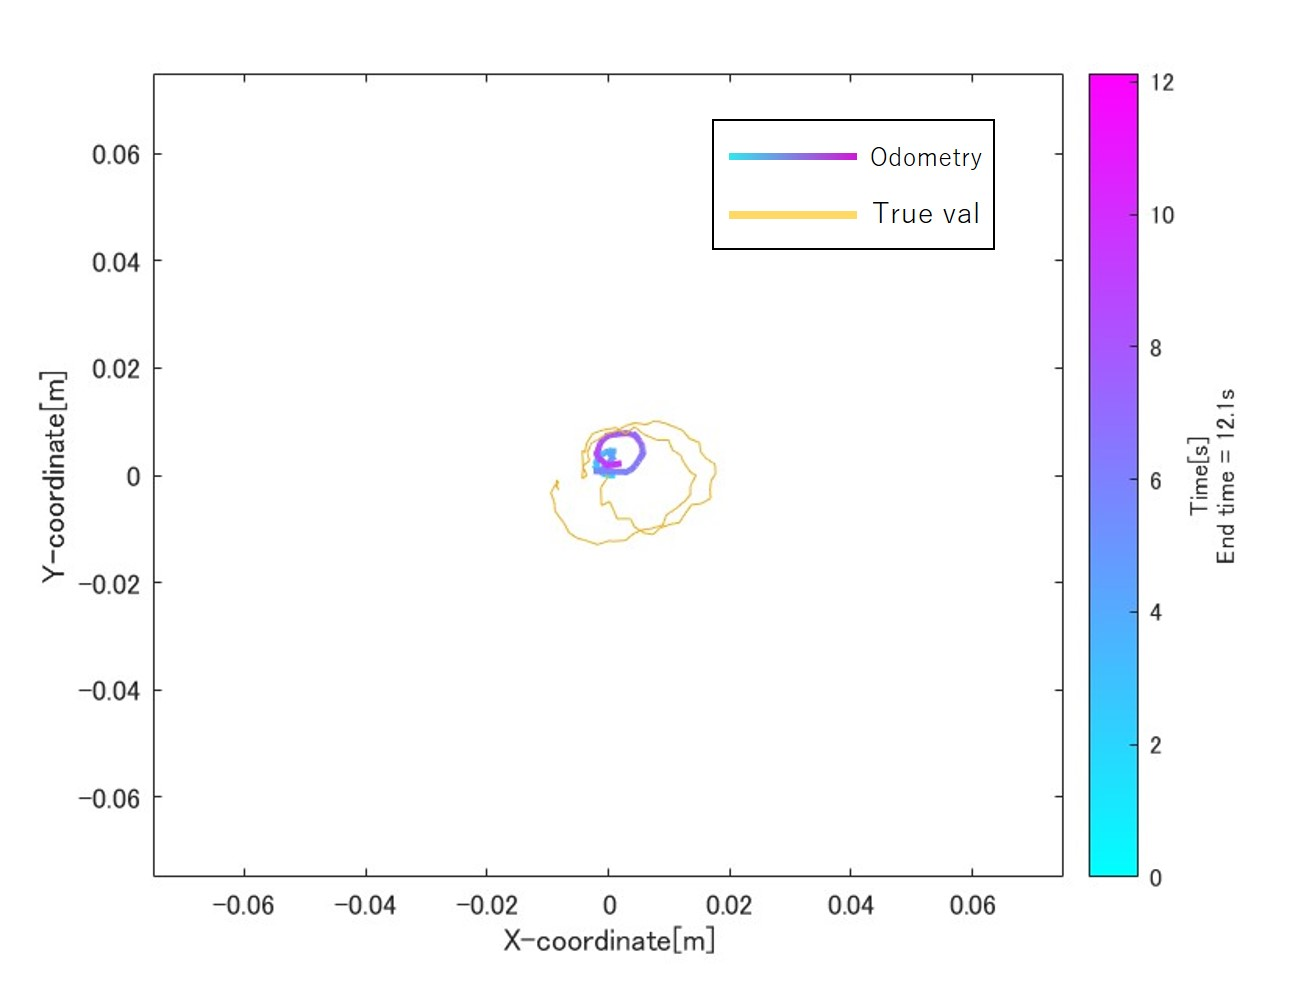
\includegraphics[width=100mm]{fig_3_2.jpg}
\caption{turning movements}
\label{fig:4}\vspace{0zh}\end{figure}

\begin{figure}[H]\centering
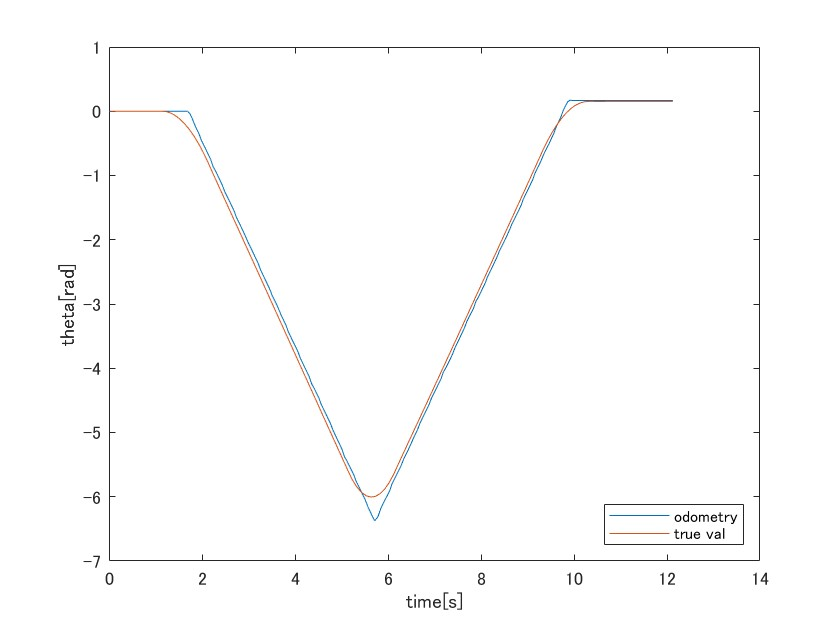
\includegraphics[width=100mm]{fig_4.jpg}
\caption{Angle Transition in turning movements}
\label{fig:5}\vspace{0zh}\end{figure}

% \begin{figure}[H]\centering
% 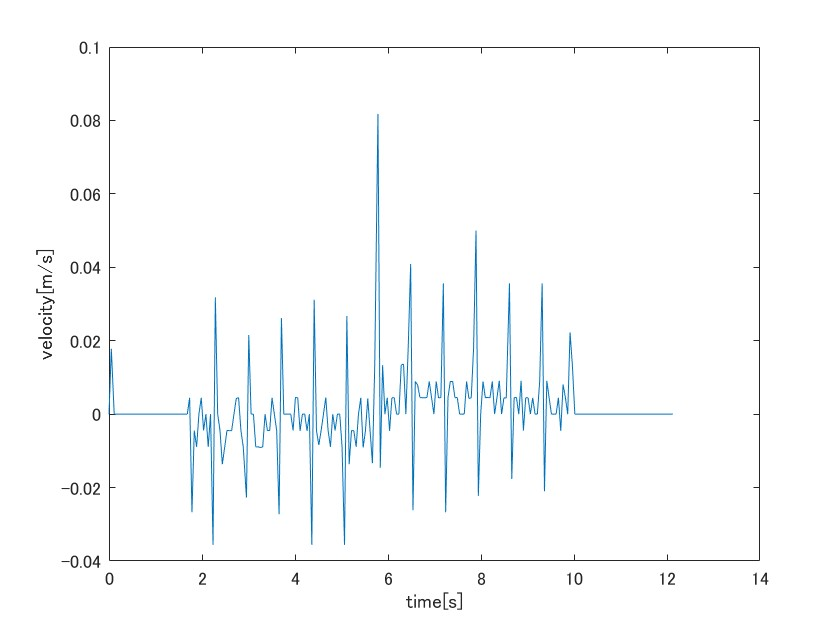
\includegraphics[width=100mm]{fig_6.jpg}
% \caption{Velocity in turning movements}
% \label{fig:6}\vspace{0zh}\end{figure}


Fig.1より直進動作において,計測終了時における進行距離の誤差は6.2mmであった.また,進行方向に対してオドメトリでは左前に進んでいることが,Fig.1より分かる.
左側にずれた距離は,最終的に183.2mmであった.また,Fig.2より真値に対して約23.5度姿勢がずれていた.
旋回動作においては.Fig.3よりほぼ誤差はなかった.最終的な誤差は,X軸方向に10.4mm,Y軸方向に3.5mmとなった.
また,Fig.4より真値とオドメトリにおける角度の誤差はほぼ無かった.

\newpage

\subsection{考察}
まず,直進動作における誤差について考察する.Fig.1より,時間経過に応じて誤差が大きくなっていることが分かる.
これは,右の車輪が滑っているためだと考えられる.右の車輪が滑ることで,左右のエンコーダー値に差が発生し,
旋回角速度とルンバの姿勢に影響する.そして,ルンバの姿勢よりオドメトリによって自己位置を算出しているため,時々刻々と誤差が蓄積し
最終的に183.2mmと大きな誤差になったのだと考えられる.\\
次に,旋回動作における誤差について考察する.旋回動作における誤差はほぼ無かった原因としては,超信地旋回時における車輪と床の摩擦が大きかったためだと考えられる.
超信地旋回時には,車輪は斜めに移動するため,車輪の接触面にかかる摩擦力の向きが分散し,車輪が空転しづらくなったのだと考えられる.





\end{document}